% move all configuration stuff into includes file so we can focus on the content
\documentclass[aspectratio=169,hyperref={pdfpagelabels=false,colorlinks=true,linkcolor=white,urlcolor=blue},t]{beamer}

%%%%%%%%%%%%%%%%%%%%%%%%%%%%%%%%%%%%%%%%%%%%%%%%%%%%%%%%%%%%%%%%%%%%%%%%%%%%%%%%%%
%%%%%%%%%%%%%%%%%%%%%%%%%%%%%%%%%%%%%%%%%%%%%%%%%%%%%%%%%%%%%%%%%%%%%%%%%%%%%%%%%%
% packages
\usepackage{pict2e}
\usepackage{epic}
\usepackage{amsmath,amsfonts,amssymb}
\usepackage{units}
\usepackage{fancybox}
\usepackage[absolute,overlay]{textpos} 
\usepackage{media9} % avi2flv: "C:\Program Files\ffmpeg\bin\ffmpeg.exe" -i TuneFreqFilterbank.avi -b 600k -s 441x324 -r 15 -acodec copy TuneFreqFilterbank.flv
\usepackage{animate}
\usepackage{gensymb}
\usepackage{multirow}
\usepackage{silence}
\usepackage[backend=bibtex,style=ieee]{biblatex}
\AtEveryCitekey{\iffootnote{\tiny}{}}
\addbibresource{references}

%%%%%%%%%%%%%%%%%%%%%%%%%%%%%%%%%%%%%%%%%%%%%%%%%%%%%%%%%%%%%%%%%%%%%%%%%%%%%%%%%%
%%%%%%%%%%%%%%%%%%%%%%%%%%%%%%%%%%%%%%%%%%%%%%%%%%%%%%%%%%%%%%%%%%%%%%%%%%%%%%%%%%
% relative paths
\graphicspath{{graph/}}


%%%%%%%%%%%%%%%%%%%%%%%%%%%%%%%%%%%%%%%%%%%%%%%%%%%%%%%%%%%%%%%%%%%%%%%%%%%%%%%%%%
%%%%%%%%%%%%%%%%%%%%%%%%%%%%%%%%%%%%%%%%%%%%%%%%%%%%%%%%%%%%%%%%%%%%%%%%%%%%%%%%%%
% units
\setlength{\unitlength}{1mm}

%%%%%%%%%%%%%%%%%%%%%%%%%%%%%%%%%%%%%%%%%%%%%%%%%%%%%%%%%%%%%%%%%%%%%%%%%%%%%%%%%%
%%%%%%%%%%%%%%%%%%%%%%%%%%%%%%%%%%%%%%%%%%%%%%%%%%%%%%%%%%%%%%%%%%%%%%%%%%%%%%%%%%
% theme & layout
\usetheme{Frankfurt}
\beamertemplatenavigationsymbolsempty
%\setbeamertemplate{frametitle}[smoothbars theme]
\setbeamertemplate{frametitle}
{
    \begin{beamercolorbox}[ht=1.8em,wd=\paperwidth]{frametitle}
        \vspace{-.1em}%
        \hspace{.2em}{\strut\insertframetitle\strut}
        
        \hspace{.2em}\small\strut\insertframesubtitle\strut
        %\hfill
        %
\includegraphics[height=.8cm,keepaspectratio]{CenterMusicTechnology-solid-2lines-white-CoAtag}
        
    \end{beamercolorbox}
    \begin{textblock*}{100mm}(11.6cm,.7cm)
        \includegraphics[height=.8cm,keepaspectratio]{logo_GTCMT_black}
    \end{textblock*}
}

% set this to ensure bulletpoints without subsections
\usepackage{remreset}
\makeatletter
\@removefromreset{subsection}{section}
\makeatother
\setcounter{subsection}{1}

%---------------------------------------------------------------------------------
% appearance
\setbeamercolor{structure}{fg=gtgold}
\setbeamercovered{transparent} %invisible
\setbeamercolor{bibliography entry author}{fg=black}
\setbeamercolor*{bibliography entry title}{fg=black}
\setbeamercolor*{bibliography entry note}{fg=black}

%\usepackage{pgfpages}
%\setbeameroption{show notes}
%\setbeameroption{show notes on second screen=right}
%---------------------------------------------------------------------------------
% fontsize
\let\Tiny=\tiny

%%%%%%%%%%%%%%%%%%%%%%%%%%%%%%%%%%%%%%%%%%%%%%%%%%%%%%%%%%%%%%%%%%%%%%%%%%%%%%%%%%
%%%%%%%%%%%%%%%%%%%%%%%%%%%%%%%%%%%%%%%%%%%%%%%%%%%%%%%%%%%%%%%%%%%%%%%%%%%%%%%%%%
% warnings
\pdfsuppresswarningpagegroup=1
\WarningFilter{biblatex}{Patching footnotes failed}
\WarningFilter{latexfont}{Font shape}
\WarningFilter{latexfont}{Some font shapes}
\WarningFilter{gensymb}{Not defining}


%%%%%%%%%%%%%%%%%%%%%%%%%%%%%%%%%%%%%%%%%%%%%%%%%%%%%%%%%%%%%%%%%%%%%%%%%%%%%%%%%%
%%%%%%%%%%%%%%%%%%%%%%%%%%%%%%%%%%%%%%%%%%%%%%%%%%%%%%%%%%%%%%%%%%%%%%%%%%%%%%%%%%
% title information
\title[]{Introduction to Audio Content Analysis}   
\author[alexander lerch]{alexander lerch} 
%\institute{~}
%\date[Alexander Lerch]{}
\titlegraphic{\vspace{-16mm}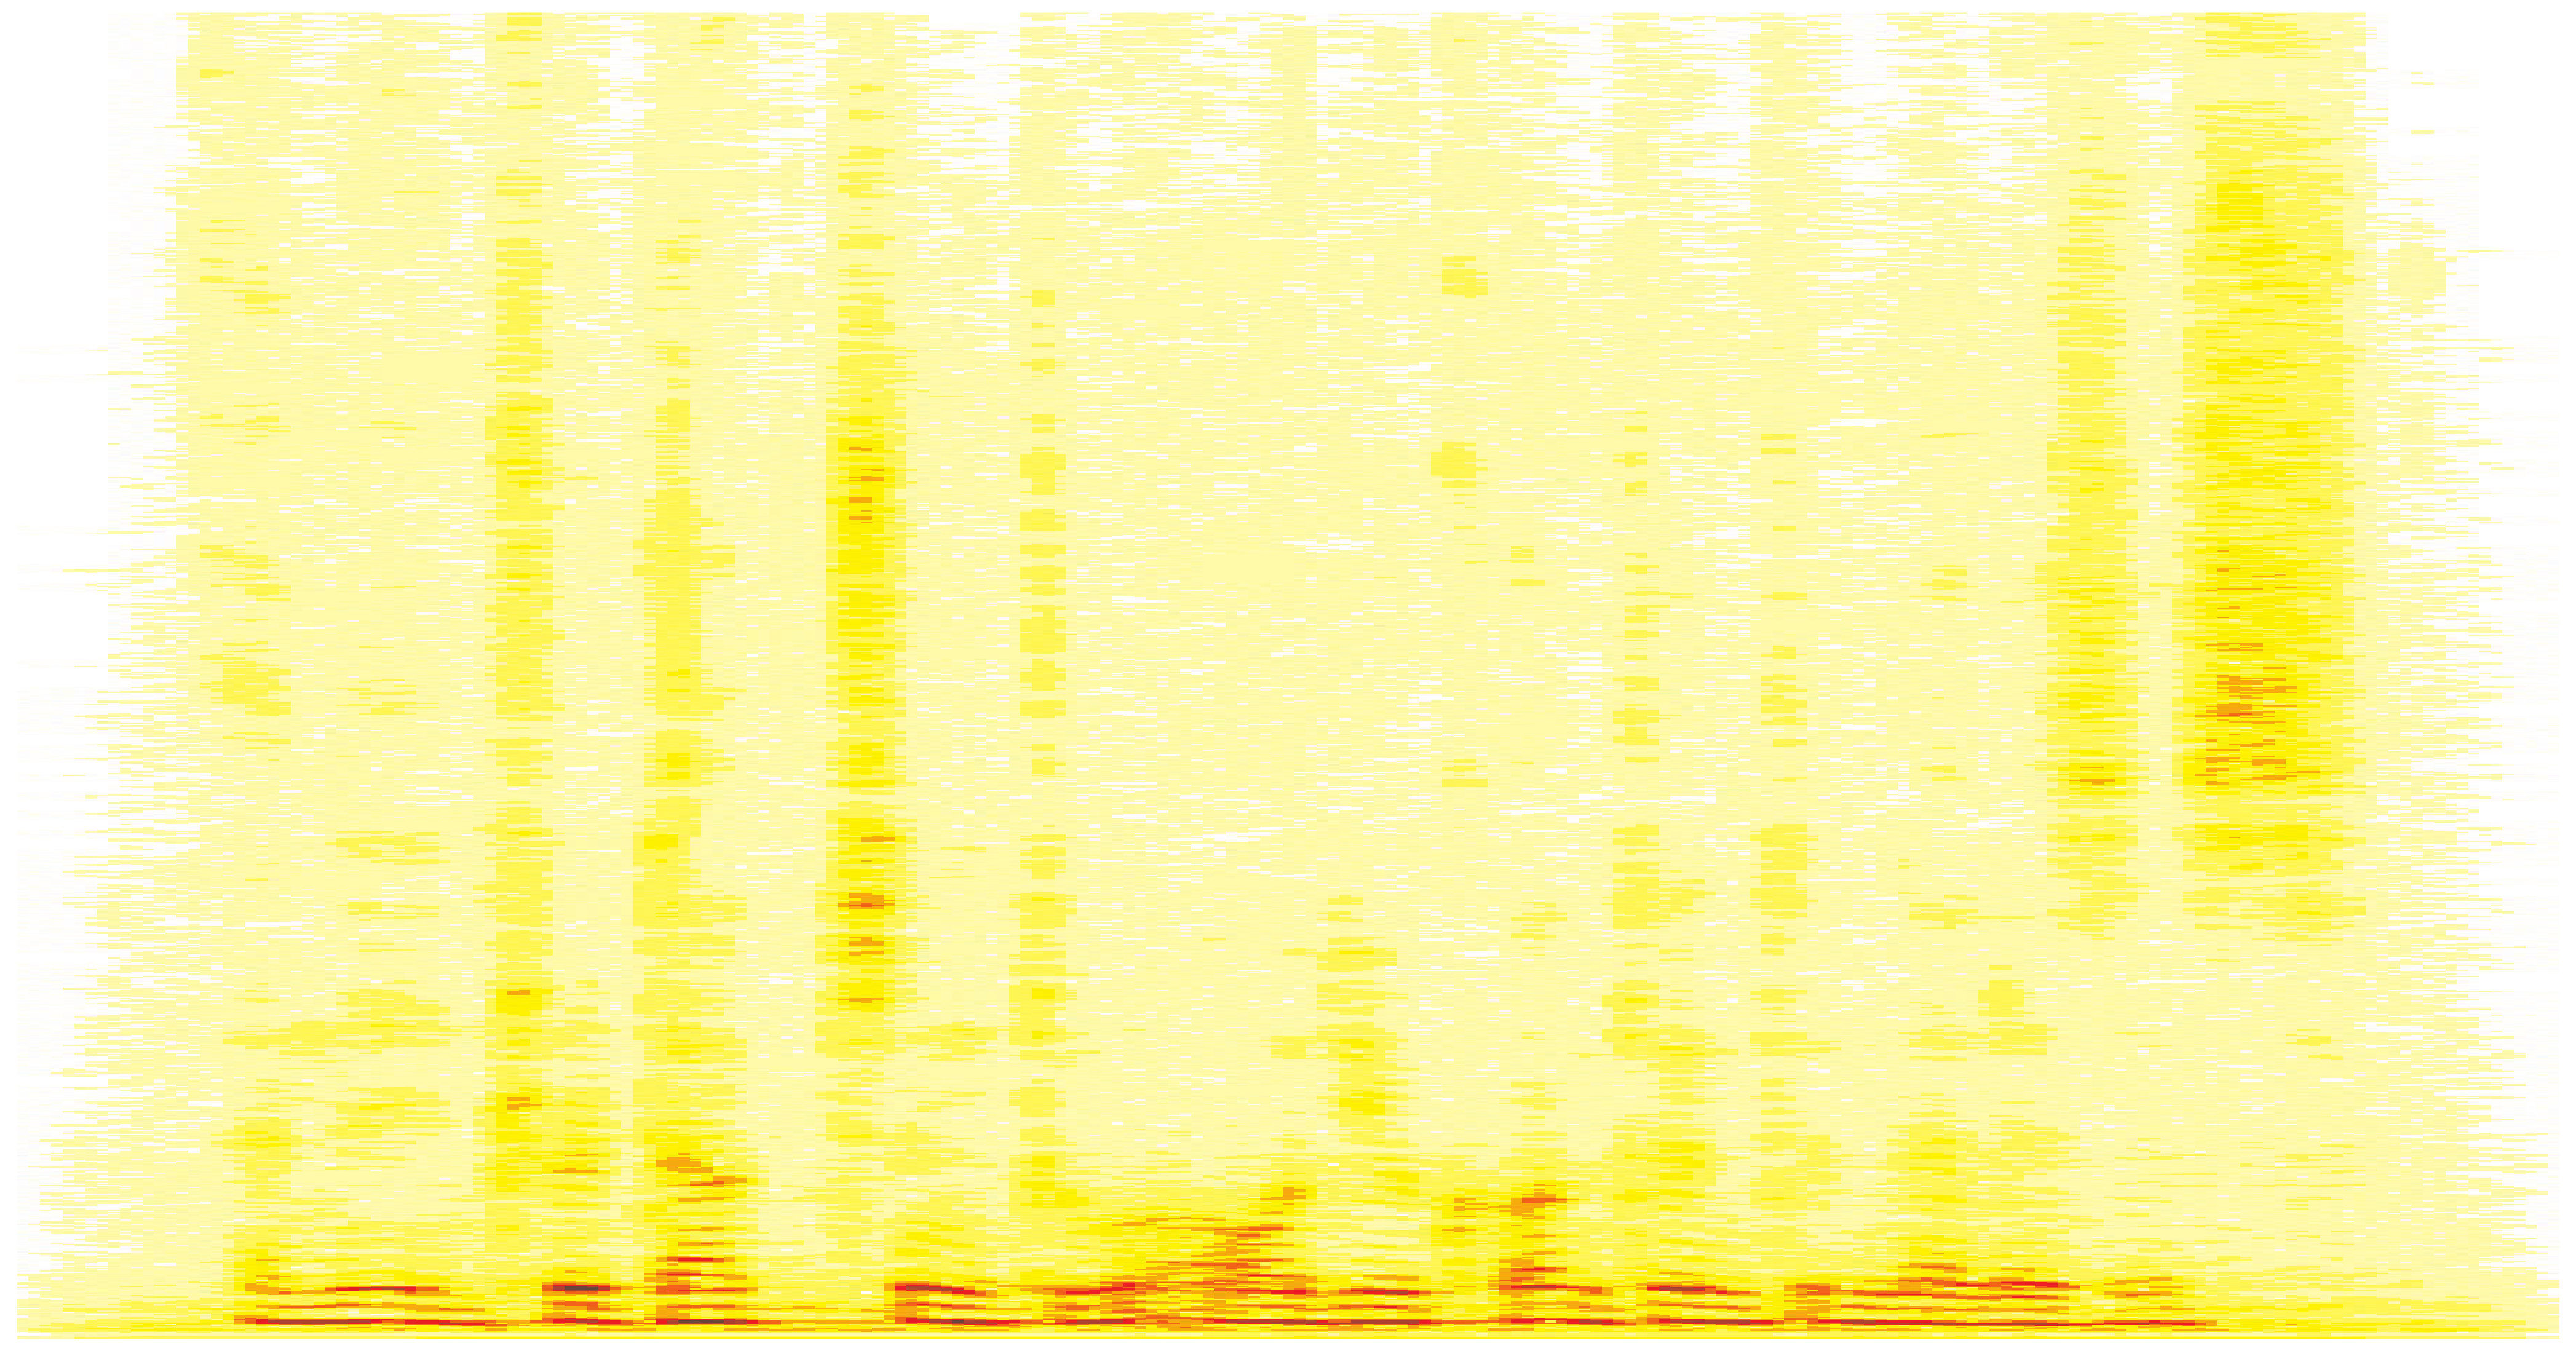
\includegraphics[width=\textwidth,height=3cm]{title}}

%%%%%%%%%%%%%%%%%%%%%%%%%%%%%%%%%%%%%%%%%%%%%%%%%%%%%%%%%%%%%%%%%%%%%%%%%%%%%%%%%%
%%%%%%%%%%%%%%%%%%%%%%%%%%%%%%%%%%%%%%%%%%%%%%%%%%%%%%%%%%%%%%%%%%%%%%%%%%%%%%%%%%
% colors
\definecolor{gtgold}{HTML}{E0AA0F} %{rgb}{0.88,0.66,1,0.06} [234, 170, 0]/256

%%%%%%%%%%%%%%%%%%%%%%%%%%%%%%%%%%%%%%%%%%%%%%%%%%%%%%%%%%%%%%%%%%%%%%%%%%%%%%%%%%
%%%%%%%%%%%%%%%%%%%%%%%%%%%%%%%%%%%%%%%%%%%%%%%%%%%%%%%%%%%%%%%%%%%%%%%%%%%%%%%%%%
% math
\DeclareMathOperator*{\argmax}{argmax}
\DeclareMathOperator*{\argmin}{argmin}
\DeclareMathOperator*{\atan}{atan}
\DeclareMathOperator*{\arcsinh}{arcsinh}
\DeclareMathOperator*{\sign}{sign}
\DeclareMathOperator*{\tcdf}{tcdf}
\DeclareMathOperator*{\si}{sinc}
\DeclareMathOperator*{\princarg}{princarg}
\DeclareMathOperator*{\arccosh}{arccosh}
\DeclareMathOperator*{\hwr}{HWR}
\DeclareMathOperator*{\flip}{flip}
\DeclareMathOperator*{\sinc}{sinc}
\DeclareMathOperator*{\floor}{floor}
\newcommand{\e}{{e}}
\newcommand{\jom}{\mathrm{j}\omega}
\newcommand{\jOm}{\mathrm{j}\Omega}
\newcommand   {\mat}[1]    		{\boldsymbol{\uppercase{#1}}}		%bold
\renewcommand {\vec}[1]    		{\boldsymbol{\lowercase{#1}}}		%bold

%%%%%%%%%%%%%%%%%%%%%%%%%%%%%%%%%%%%%%%%%%%%%%%%%%%%%%%%%%%%%%%%%%%%%%%%%%%%%%%%%%
%%%%%%%%%%%%%%%%%%%%%%%%%%%%%%%%%%%%%%%%%%%%%%%%%%%%%%%%%%%%%%%%%%%%%%%%%%%%%%%%%%
% media9
\newcommand{\includeaudio}[1]{{\includemedia[
                        addresource=audio/#1.mp3,
                        width=5mm,
                        height=5mm,
                        activate=onclick,
                        flashvars={
                            source=audio/#1.mp3  
                            &autoPlay=true
                        }]
                        {
\includegraphics[width=5mm, height=5mm]{SpeakerIcon}}
                        {APlayer.swf}}}
\newcommand{\audioautoplay}[1]{{\begin{center}\includemedia[
                            addresource=audio/#1.mp3,
                            width=.1\linewidth,
                            height=.01\linewidth,
                            activate=pageopen,
                            flashvars={
                                source=audio/#1.mp3  
                                &autoPlay=true
                            }]
                            {}
                            {APlayer.swf}\end{center}}}

\newcommand{\includevideo}[1]{{\begin{center}\includemedia[
                        addresource=video/#1.mp4,
                        width=0.8\linewidth,
                        height=0.4\linewidth,
                        activate=onclick,
                        flashvars={
                            source=video/#1.mp4  
                            &autoPlay=true
                        }]
                        {}
                        {VPlayer.swf}\end{center}}}
\newcommand{\videowithmatlab}[1]{{\begin{center}\includemedia[
                        addresource=video/animate#1.mp4,
                        width=0.8\linewidth,
                        height=0.4\linewidth,
                        activate=onclick,
                        flashvars={
                            source=video/animate#1.mp4  
                            &autoPlay=true
                        }]
                        {}
                        {VPlayer.swf}\end{center}\addreference{matlab source: matlab/animate#1.m}}}
                        

%%%%%%%%%%%%%%%%%%%%%%%%%%%%%%%%%%%%%%%%%%%%%%%%%%%%%%%%%%%%%%%%%%%%%%%%%%%%%%%%%%
%%%%%%%%%%%%%%%%%%%%%%%%%%%%%%%%%%%%%%%%%%%%%%%%%%%%%%%%%%%%%%%%%%%%%%%%%%%%%%%%%%
% other commands
\newcommand{\question}[1]{%\vspace{-4mm}
                          \setbeamercovered{invisible}
                          \begin{columns}[T]
                            \column{.8\textwidth}
                                \textbf{#1}
                            \column{.2\textwidth}
                                \vspace{-8mm}
                                \begin{flushright}
                                     
\includegraphics[scale=.5]{question_mark}
                                \end{flushright}
                                \vspace{6mm}
                          \end{columns}\pause\vspace{-12mm}}

\newcommand{\toremember}[1]{%\vspace{-4mm}
                          \begin{columns}[T]
                            \column{.8\textwidth}
                                \textbf{#1}
                            \column{.2\textwidth}
                                \vspace{-4mm}
                                \begin{flushright}
                                     
\includegraphics[scale=.5]{exclamation_mark}
                                \end{flushright}
                                \vspace{6mm}
                          \end{columns}\vspace{-6mm}}

\newcommand{\matlabexercise}[1]{%\vspace{-4mm}
                          \setbeamercovered{invisible}
                          \begin{columns}[T]
                            \column{.8\textwidth}
                                \textbf{matlab exercise}: #1
                            \column{.2\textwidth}
                                \begin{flushright}
                                     
\includegraphics[scale=.5]{logo_matlab}
                                \end{flushright}
                                %\vspace{6mm}
                          \end{columns}}

\newcommand{\addreference}[1]{  
                  
                    \begin{textblock*}{\baselineskip }(1.12\textwidth,.3\textheight) %(1.15\textwidth,.4\textheight)
                        \rotatebox{90}{\tiny {#1}}
                    \end{textblock*}}
                    
\newcommand{\figwithmatlab}[1]{
                    \begin{figure}
                        \centering
                        \includegraphics{#1}
                        %\label{fig:#1}
                    \end{figure}
                    
                    \addreference{matlab source: \href{https://github.com/alexanderlerch/ACA-Slides/blob/master/matlab/display#1.m}{matlab/display#1.m}}}
\newcommand{\figwithref}[2]{
                    \begin{figure}
                        \centering
                        \includegraphics{#1}
                        \label{fig:#1}
                    \end{figure}
                    
                    \addreference{#2}}  
                                    
\newcommand{\inserticon}[1]{

                    \begin{textblock*}{100mm}(14.5cm,7.5cm)
                        \includegraphics[height=.8cm,keepaspectratio]{#1}
                    \end{textblock*}}            

%%%%%%%%%%%%%%%%%%%%%%%%%%%%%%%%%%%%%%%%%%%%%%%%%%%%%%%%%%%%%%%%%%%%%%%%%%%%%%%%%%
%%%%%%%%%%%%%%%%%%%%%%%%%%%%%%%%%%%%%%%%%%%%%%%%%%%%%%%%%%%%%%%%%%%%%%%%%%%%%%%%%%
% counters
\newcounter{i}
\newcounter{j}
\newcounter{iXOffset}
\newcounter{iYOffset}
\newcounter{iXBlockSize}
\newcounter{iYBlockSize}
\newcounter{iYBlockSizeDiv2}
\newcounter{iDistance}



\subtitle{Module 2.4: Fundamentals~---~Blocking}

%%%%%%%%%%%%%%%%%%%%%%%%%%%%%%%%%%%%%%%%%%%%%%%%%%%%%%%%%%%%%%%%%%%%%%%%%%%%
\begin{document}
    % generate title page
	

\begin{frame}
    \titlepage
    %\vspace{-5mm}
    \begin{flushright}
        \href{http://www.gtcmt.gatech.edu}{\includegraphics[height=.8cm,keepaspectratio]{logo_GTCMT_black}}
    \end{flushright}
\end{frame}


    \section[overview]{lecture overview}
        \begin{frame}{introduction}{overview}
            \begin{block}{corresponding textbook section}
                    \href{http://ieeexplore.ieee.org/xpl/articleDetails.jsp?tp=&arnumber=6331119&}{Chapter 2~---~Fundamentals}: pp.~18--20
            \end{block}

            \begin{itemize}
                \item   \textbf{lecture content}
                    \begin{itemize}
                        \item   splitting the audio signal into blocks
                        \item   block length and hop size
                    \end{itemize}
                \bigskip
                \item<2->   \textbf{learning objectives}
                    \begin{itemize}
                        \item   describe the reasons for blocking
                        \item   summarize the principle using the correct terminology
                    \end{itemize}
            \end{itemize}
            \inserticon{directions}
        \end{frame}

   \section[blocking]{block-based processing}
        \begin{frame}{block based processing}{introduction}
            \begin{itemize}
                \item   typical audio applications \textbf{process blocks} of audio data  
                \item   instead of having a function called per sample, it is called with block of samples
                \bigskip
                \item   \textbf{reasons}:
                    \begin{itemize}
                        \item   block based processing methods such as the Short-Time Fourier Transform
                        \item	quasi-stationary signal properties within block
                        \item	audio hardware characteristics (real-time systems)
                        \item	efficiency (memory allocation, SIMD)
                    \end{itemize}
                \smallskip
                \item<2->   typical block lengths:
                    \begin{itemize}
                        \item   1\ldots thousands of samples
                        \item   often powers of 2
                    \end{itemize}
            \end{itemize}
        \end{frame}
        \begin{frame}{block based processing}{description}
            \vspace{-4mm}
            \figwithmatlab{Blocking}
            \pause
            \begin{columns}
                \column{.6\textwidth}
                    \vspace{-11mm}
                    \begin{figure}
                        \centering
                        \begin{footnotesize}
				\begin{picture}(60,40)
					\setcounter{iXOffset}{0}
					\setcounter{iYOffset}{24}
					\setcounter{iXBlockSize}{16}
					\setcounter{iYBlockSize}{4}
					\setcounter{iYBlockSizeDiv2}{2}
					\setcounter{iDistance}{8}

					% block indices
					\put(\value{iXOffset}, \value{iYOffset})
						{\text{{\shortstack[c]{$n$}}}}
					\addtocounter{iYOffset}{-\value{iYBlockSize}}
					\addtocounter{iYOffset}{-\value{iYBlockSizeDiv2}}
					\put(\value{iXOffset}, \value{iYOffset})
						{\text{{\shortstack[c]{$n+1$}}}}
					\addtocounter{iYOffset}{-\value{iYBlockSize}}
					\addtocounter{iYOffset}{-\value{iYBlockSizeDiv2}}
					\put(\value{iXOffset}, \value{iYOffset})
						{\text{{\shortstack[c]{$n+2$}}}}
					\addtocounter{iYOffset}{-\value{iYBlockSize}}
					\addtocounter{iYOffset}{-\value{iYBlockSizeDiv2}}
					\put(\value{iXOffset}, \value{iYOffset})
						{\text{{\shortstack[c]{$n+3$}}}}

					% audio time line
					\setcounter{iYOffset}{30}
					\setcounter{iXOffset}{5}
					\put(\value{iXOffset}, \value{iYOffset})
						{\vector(1,0){50}}
	
					% blocks
					\addtocounter{iXOffset}{5}
					\addtocounter{iYOffset}{-\value{iYBlockSize}}
					\addtocounter{iYOffset}{-\value{iYBlockSizeDiv2}}
					\put(\value{iXOffset}, \value{iYOffset})
						{\framebox(\value{iXBlockSize}, \value{iYBlockSize})}
					\addtocounter{iXOffset}{5}
					\addtocounter{iYOffset}{-\value{iYBlockSize}}
					\addtocounter{iYOffset}{-\value{iYBlockSizeDiv2}}
					\put(\value{iXOffset}, \value{iYOffset})
						{\framebox(\value{iXBlockSize}, \value{iYBlockSize})}
					\addtocounter{iXOffset}{5}
					\addtocounter{iYOffset}{-\value{iYBlockSize}}
					\addtocounter{iYOffset}{-\value{iYBlockSizeDiv2}}
					\put(\value{iXOffset}, \value{iYOffset})
						{\framebox(\value{iXBlockSize}, \value{iYBlockSize})}
					\addtocounter{iXOffset}{5}
					\addtocounter{iYOffset}{-\value{iYBlockSize}}
					\addtocounter{iYOffset}{-\value{iYBlockSizeDiv2}}
					\put(\value{iXOffset}, \value{iYOffset})
						{\framebox(\value{iXBlockSize}, \value{iYBlockSize})}

	
					% lengths
					\linethickness{.03mm}
					\setcounter{iYOffset}{34}
					\setcounter{iXOffset}{10}
					\put(\value{iXOffset}, \value{iYOffset})
						{\line(0,-1){12}}
					\put(\value{iXOffset}, \value{iYOffset})
						{\vector(1,0){1}}
					\addtocounter{iXOffset}{5}
					\put(\value{iXOffset}, \value{iYOffset})
						{\line(0,-1){18}}
					\put(\value{iXOffset}, \value{iYOffset})
						{\vector(-1,0){1}}
					\addtocounter{iXOffset}{5}
					\addtocounter{iXOffset}{5}
					\put(\value{iXOffset}, \value{iYOffset})
						{\line(0,-1){30}}
					\put(\value{iXOffset}, \value{iYOffset})
						{\vector(1,0){1}}
					\addtocounter{iXOffset}{\value{iXBlockSize}}
					\put(\value{iXOffset}, \value{iYOffset})
						{\line(0,-1){30}}
					\put(\value{iXOffset}, \value{iYOffset})
						{\vector(-1,0){1}}

					\put(11, 34)
						{\text{$\mathcal{H}$}}
					\put(32, 34)
						{\text{$\mathcal{K}$}}
					\put(56, 28)
						{\text{$i$}}
				\end{picture}
\end{footnotesize}
	
                    \end{figure}
                \column{.4\textwidth}
                    \begin{itemize}
                        \item   $\mathcal{K}$: block length
                        \item   $\mathcal{H}$: hop size
                        \item   $n$: block index
                        \item   $i$: sample index
                    \end{itemize}
            \end{columns}
        \end{frame}
    \section[definitions]{terms \& definitions}
        \begin{frame}{block based processing}{terms and definitions}
            \begin{columns}
                \column{.75\textwidth}
                    \begin{itemize}
                        \item   \textbf{block boundaries}:
                            \begin{eqnarray*}
                                i_{\mathrm{s}}(n)	&=& i_{\mathrm{s}}(n-1) + \mathcal{H}\\
                                i_{\mathrm{e}}(n)		&=& i_{\mathrm{s}}(n) + \mathcal{K} - 1
                            \end{eqnarray*}
                        \item   \textbf{overlap ratio}:
                            \begin{equation*}
                                o_{\mathrm{r}}	= \frac {\mathcal{K}-\mathcal{H}}{\mathcal{K}}
                            \end{equation*}
                        \item   \textbf{time stamp}:
                            \begin{equation*}
                                t_{\mathrm{s}}(n) = \frac{i_{\mathrm{e}}(n)-i_{\mathrm{s}}(n)+1}{2\cdot f_{\mathrm{S}}} + \frac{i_{\mathrm{s}}(n)}{f_{\mathrm{S}}} = \frac{\mathcal{K}}{2\cdot f_{\mathrm{S}}} + \frac{i_{\mathrm{s}}(n)}{f_{\mathrm{S}}} 
                            \end{equation*}
                    \end{itemize}
                \column{.25\textwidth}
                    \begin{itemize}
                        \item   $\mathcal{K}$: block length
                        \item   $\mathcal{H}$: hop size
                        \item   $n$: block index
                        \item   $i$: sample index
                        \item   $f_\mathrm{S}$: sample rate
                    \end{itemize}
            \end{columns}
        \end{frame}	

    \section{summary}
        \begin{frame}{summary}{lecture content}
            \begin{itemize}
                \item   \textbf{audio signal is typically split into blocks}
                \item   each block processed individually
                \smallskip
                \item   \textbf{terms}:
                    \begin{itemize}
                        \item   \textit{block length}:
                            \begin{itemize}
                                \item minimum: $1$
                                \item   typical: $256 \ldots 16384$
                            \end{itemize}
                        \item   \textit{hop size}:
                            \begin{itemize}
                                \item minimum: $1$
                                \item   maximum: block length
                                \item   typical: half of block length
                            \end{itemize}
                        \item   block \textit{time stamp}:
                            \begin{itemize}
                                \item typically refers to middle of block
                            \end{itemize}
                    \end{itemize}
            \end{itemize}
            \inserticon{summary}
        \end{frame}
\end{document}
